%%%%%%%%%%%%%%%%%%%%%%%%%%%%%%%%%%%%%%%%%%%%%%%%%%%%%%%%%%%%%%%%%%%%%%%%%%%
%   导言区
\documentclass[12pt, a4paper, oneside]{ctexart}
\usepackage{amsmath, amsthm, amssymb, appendix, cite}
\usepackage{bm, graphicx, hyperref, mathrsfs, geometry}

\newcommand{\upcite}[1]{\textsuperscript{\cite{#1}}}

\title{\textbf{伪卫星技术与应用的学习报告}}

\date{\today}
%\advisor{}

\linespread{1.45}    %设置{n}倍行距
\geometry{left=2.5cm, right=2.5cm, top=2.0cm, bottom=2.0cm}%设定页边距
%%%%%%%%%%%%%%%%%%%%%%%%%%%%%%%%%%%%%%%%%%%%%%%%%%%%%%%%%%%%%%%%%%%%%%%%%%%
\begin{document}

\maketitle

\setcounter{page}{1}
\maketitle
\thispagestyle{empty}
\begin{center}
    \rule[-10pt]{16cm}{0.05em}
\end{center}%一条不错的加横线指令
%%%%%%%%%%%%%%%%%%%%%%%%%%%%%%%%%%%%%%%%%%%%%%%%%%%%%%%%%%%%%%%%%%%%%%%%%%%
%   添加摘要、关键词
\begin{abstract}
    随着北斗三号系统全面投入使用,现如今的全球卫星导航系统(GNSS)已经在测量、测绘、测地、定位、导航等方面得到了广泛运用并引起了一轮轮学科革命,并极大地便利着人们的日常生活。与此同时,完全基于卫星的导航定位系统具有的内在缺点也逐渐显现出来:信号衰减与定位精度受限于卫星的几何布局。因此,在比较苛刻的观测条件下(例如高楼众多的城市中央、墙壁错综复杂的室内、受地形阻挡视野的隧道或矿井或者远离地球的星球表面)定位效果急剧下降。然而,伪卫星技术的发展与应用补全了这一不足。本文记录了作者在学习伪卫星技术过程中对其发展历程、应用场景和关键技术的总结与联想。
    \par\textbf{关键词:}卫星导航;卫星定位;伪卫星;室内定位;GNSS;北斗;综述;学习报告. 
\end{abstract}
\begin{center}
    \rule[-10pt]{16cm}{0.05em}
\end{center}%一条不错的加横线指令
%%%%%%%%%%%%%%%%%%%%%%%%%%%%%%%%%%%%%%%%%%%%%%%%%%%%%%%%%%%%%%%%%%%%%%
%   正文编排
\section{概述}

伪卫星是指在地球大气层内或者以上的空间建立的信号发射器,他们使用与GPS等卫星导航系统相同的频段来发射信号,并实时接收GPS信号,从而修正伪距误差,起到类似一颗真正的卫星的作用,所以称为“伪”卫星。\upcite{07}伪卫星可以通过多种方式制造,可以在固定的坐标上建设信号发射站充当固定的伪卫星信号源,又例如通过发射气球或高空飞机,或者通过将卫星级设备安装在无人驾驶飞机或火箭上发射到太空。

伪卫星具有体积小、成本低和操作简单的优势,可以满足多种应用需求。例如,伪卫星可以用于地面监测、环境观测、气象预报等遥感应用;可以提供宽带互联网服务、移动通信服务和卫星电视服务等通信应用;可以提供全球定位服务、航空定位服务和海上导航服务等导航应用;还可以用于天文观测、空间环境监测等其他领域。\upcite{05,07}


但是有时它们并不像真正的卫星那样稳定,也不具有长期的使用寿命。伪卫星技术的发展主要是为了满足短期的、或者是在某些地区的临时的需求,或者是为了补充真正的卫星在某些情况下无法提供的服务,例如室内的分米级以上精度定位、隧道等地形阻挡下的持续导航、火星车在火星表面的行驶等。\upcite{01,001}

本篇学习报告旨在列出伪卫星技术的发展现状和应用前景,并对相关研究进行分类、比较和总结。
\lable{??}

\section{资料综述}

\subsection{伪卫星技术的发展}

伪卫星技术的发展可以追溯到20世纪50年代,但直到近年才得到大规模应用。随着小型卫星技术的不断提升和成本的降低,伪卫星的发射数量迅速增加。根据统计,截至2022年,全球已有超过10000颗伪卫星发射升空。\upcite{07}

GPS开发初期,采用4台地面发射机来提供模拟GPS信号以对接收机进行校验,其发送伪卫星位置L1频率固定坐标。其后,GALILEO系统在技术验证阶段也使用了验证频率分配与用户社会,这就是伪卫星导航技术的雏形。

\begin{figure}[ht]
  \centering
  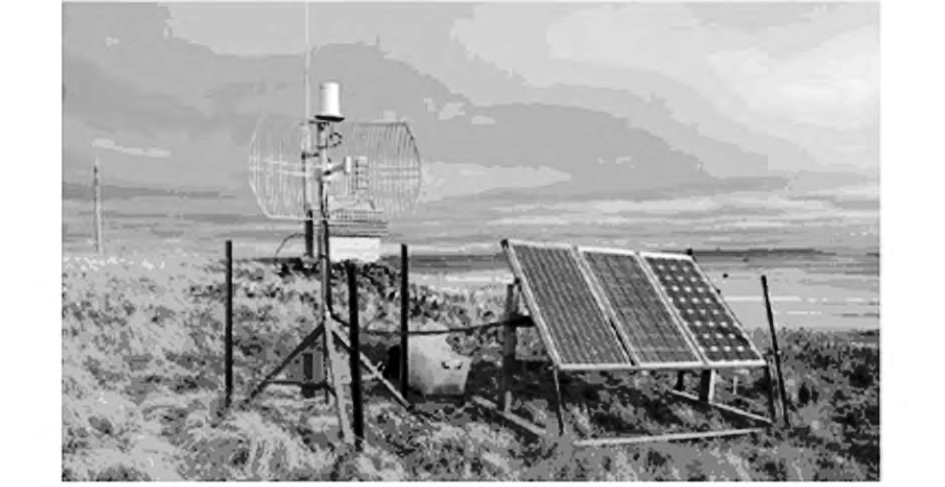
\includegraphics[width=0.65\textwidth]{img/wei.png}
  \caption{伪卫星示意图}
  \label{yuanjian}
\end{figure}

使用伪卫星定位和导航首先由Beser{\&}Par-kinson(1982)和Klein{\&}Parkinson(1984)提出。80年代中期海运无线电技术委员会(RTCM)给伪卫星下了以下定义:可以接收GPS信号,计算伪距及伪距率,并且L波段修正后的信号每秒50位,另外伪卫星传输的信号一定要与GPS相似,同时要防止对GPS等设备的干扰。然而当时伪卫星原型的设计成本很高,约10万至20万美元。

90年代初期斯坦福大学学者研究出一种低价位GPS L1C/A码伪卫星应用于第三类自动进场系统中。20世纪90年代中,最早的商业伪卫星制造商Integri Nautics公司应运而生。随后十年间,市场上出现了几家伪卫星生产商。在硬件设计不断改进的情况下,伪卫星在许多领域都得到了推广应用。\upcite{001}

\subsection{伪卫星技术的应用}

与GNSS导航卫星的功能和原理一样,伪卫星主要包括接收机、发射机、天线这几部分,并且能发送与导航卫星相同格式的导航电文。\upcite{05}根据实现目的的不同,伪卫星导航定位应用主要分为:增强GPS的伪卫星系统、独立定位的伪卫星系统、参与组合导航的伪卫星系统三种。\upcite{002}

\subsubsection{增强GPS的伪卫星系统}

在一些特殊场所,如密集城市、矿井、露矿、峡谷、高边坡区、隧道,受GPS卫星受地形遮挡影响,视野内数量有限,卫星分布图差,GPS导航定位精度不高,甚至不能保证导航定位需要。\upcite{01}为此需在局部高精度GPS定位地区周围设置多个伪卫星站,同时发射GPS卫星信号及差分校正。此时伪卫星的作用是辅助衰减严重的GPS卫星信号,让用户在使用GPS接收机对上述信号进行接收时,大大改善卫星的几何图形结构,还可以提高整个系统导航定位的精度,从而使GPS导航定位系统具有良好的性能。\upcite{002,06}

\begin{figure}[ht]
  \centering
  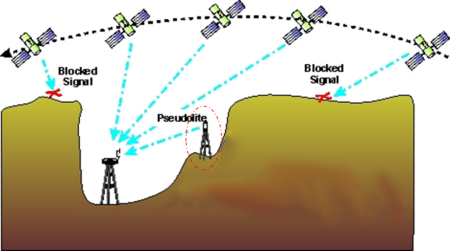
\includegraphics[width=0.65\textwidth]{img/shiyitu.png}
  \caption{地形阻挡下伪卫星增强GPS示意图\upcite{09}}
  \label{}
\end{figure}

例如,当前GNSS系统已经广泛用于农林渔业、水文监测、电力调配、防灾减灾、地质测绘、通信授时、气象监测、公共安全等领域。但在公路隧道内,视野面积被山体大范围阻挡,GPS信号难以被接收到,往往形成“信号盲区”,而传统的光学定位、Wi-Fi定位、UWB定位、蓝牙定位等方式存在效率低、精度差、可靠性欠缺、终端可移植性不佳等问题,这对隧道内车流的监控、调度,隧道内高精度要求施工,以至于“智慧公路”的建设是不利的。此时我们可以在隧道两端、沿隧道基线设置卫星测站,解算出测站精确坐标,并在隧道内部设置一系列伪卫星基站。有了这些伪卫星与基线两端测站计算出的相对坐标,就可以使用“伪距差分法”测算出接收机的精确位置。\upcite{04,01}

\begin{figure}[ht]
  \centering
  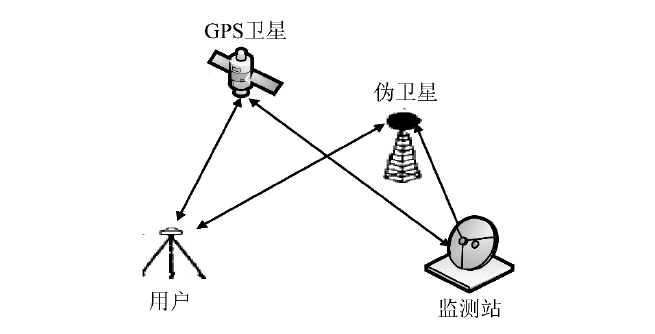
\includegraphics[width=0.70\textwidth]{img/1.png}
  \caption{增强GPS的伪卫星系统示意图\upcite{002}}
  \label{}
\end{figure}

\subsubsection{独立定位的伪卫星系统}

例如,随着无线网络与移动通信技术的快速发展,基于定位的服务(Location-Based Service,LBS)被广泛应用于室内,如大型超市,会场,矿井等等,关键在于对移动终端(Mobile terminal,MT)进行精确定位,从而实现多种应用,如医院内部病床、人力的调配,商场中商品的位置信息服务,或地下停车场的智能寻路等。\upcite{11,12,06}可以预见,未来伪卫星技术在室内的应用将大大促进智能化潮流的推进。

\begin{figure}[ht]
  \centering
  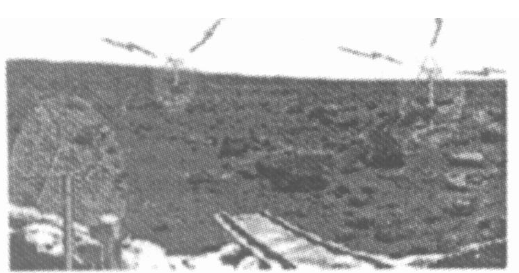
\includegraphics[width=0.70\textwidth]{img/huoxing.png}
  \caption{火星表面伪卫星阵列\upcite{001}}
  \label{}
\end{figure}

更进一步,伪卫星技术甚至可以应用于远离地球的其他星球表面。\upcite{001}在遥远的火星表面上,难以接受到GPS信号,这时伪卫星的基准站位置将难以精确地测出,火星车的定位与导航就成为了一个难题。为此,,斯坦福大学空间机器人实验室提出了一种新的伪卫星定位系统——自校准伪卫星阵列(SCPA)。该系统的所有伪卫星都是收发器,能够同时发射并接收系统中其他伪卫星的信号,并利用差分技术,仅仅依靠阵列内的伪卫星、在没有独立参考站的情况下消除每一对接收器和发射器之间的钟差。最终这套系统的定位精度达到了厘米级。\upcite{lemaster1998mars}

\begin{figure}[ht]
  \centering
  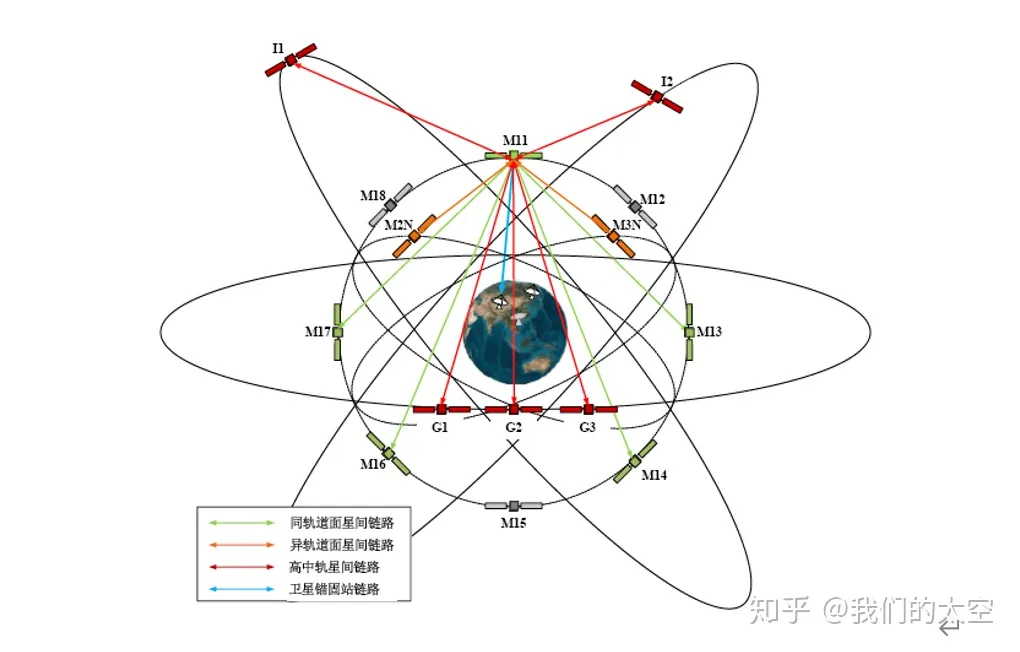
\includegraphics[width=0.70\textwidth]{img/xjll.png}
  \caption{北斗三号使用的星间链路技术大大提高了系统的精度和抗性}
  \label{}
\end{figure}

\begin{itemize}
\item 这一思想同样体现在我国北斗三号全球卫星导航系统的建设上。在地面基准站难以遍布全球的现实背景下,北斗三号各星之间相互组网,配合“天链”通信卫星网络,形成了类似SCPA的网络,不仅减少了所需的地面基准站数量,还大大提高了北斗三号的定位精度。\upcite{13}
\end{itemize}

\begin{figure}[ht]
  \centering
  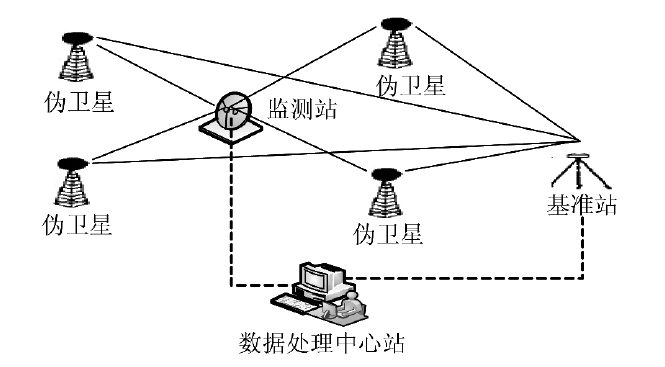
\includegraphics[width=0.70\textwidth]{img/2.png}
  \caption{独立定位的伪卫星系统示意图\upcite{002}}
  \label{}
\end{figure}

\subsubsection{参与组合导航的伪卫星系统}

组合导航的集成方式有多种,其中卫星导航系统可与卫星导航系统集成(GPS/GLONASS、GPS/BDS、GPS/BDS/GLONASS),卫星导航可与惯性导航(Inertial Navigation System, INS)集成(GPS/INS),卫星导航可与伪卫星集成(也即前文提到的伪卫星增强的GPS)。\upcite{002}

\begin{figure}[ht]
  \centering
  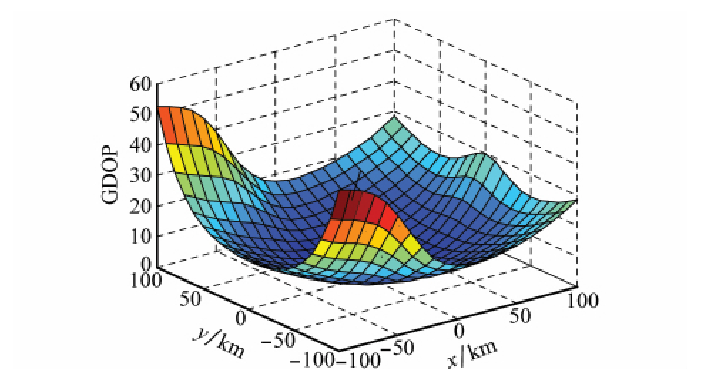
\includegraphics[width=0.65\textwidth]{img/fz.png}
  \caption{伪卫星系统参与组合导航的仿真结果\upcite{03}}
  \label{}
\end{figure}

例如,当我们单独使用INS系统时,其加速度计产生的误差可随时间累积。一般情况下,可以周期性地使用与卫星导航系统的通信来准确订正INS的系统误差,但在如上文和摘要提到的恶劣环境下,卫星信号可能长时间无法接收到或是衰减严重,长时间之后,集成的导航系统的性能将大幅下降甚至全面失真。\upcite{14}这时就要充分发挥伪卫星系统体积小、灵活性好的优势,建立一套集成GNSS/INS/伪卫星系统的组合导航系统。\upcite{002,14}运用这种组合导航系统,卫星导航定位的准确性和可靠性都能够得到大幅提升。事实上这一种技术已经在各种终端上得到应用。例如,现时我们的手机终端就集成了GNSS终端、LBS基站定位终端、惯性导航组件,当我们利用手机导航驾车进入隧道,虽然GNSS信号难以接受到,但是如果利用伪卫星技术与上述终端进行组合,便可以实现在隧道内的持续导航。\upcite{01,14,15}

\begin{figure}[ht]
  \centering
  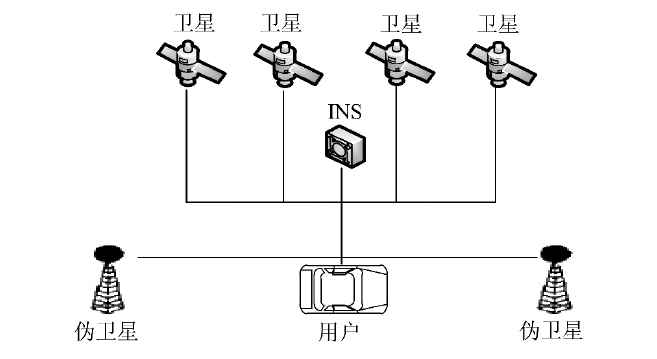
\includegraphics[width=0.70\textwidth]{img/3.png}
  \caption{参与组合导航的伪卫星系统示意图\upcite{002}}
  \label{}
\end{figure}

\subsection{伪卫星应用中的关键技术}

由于伪卫星本身处在大气层中,而且本身体积较小,且常常应用于比较狭小逼仄的环境中,所以除了系统本身的时钟误差、与卫星导航系统的同步、收发机的信号衰减等内在问题,还会产生远近效应、多径效应、大气层时延等问题,这也是伪卫星技术优化应用的关键所在。\upcite{001,002}

\subsubsection{远-近效应}

伪卫星技术中远-近效应就是说,在近处GPS信号被大量伪卫星发射信号淹没,而在远处伪卫星信号则衰减迅速、难以接收到。求解伪卫星远距—近距的主要途径有:调频;轨迹约束;设计天线方向图;采用分立天线;带外发射;选择新型扩频码;频率偏移等;脉冲发射等等。\upcite{03}其中比较实用的是脉冲发射法(或“时间分割调制”方案),也就是通过周期性短时间发射,只占用较小一段时间来传送伪卫星信号。研究发现在伪卫星占空比仅为10\%时,伪卫星信号就容易被接收到,且导航卫星平均负增益不超过1dB,并且在接下来的90\%时间中均可接收到卫星导航信号。\upcite{001,002}

\begin{figure}[ht]
  \centering
  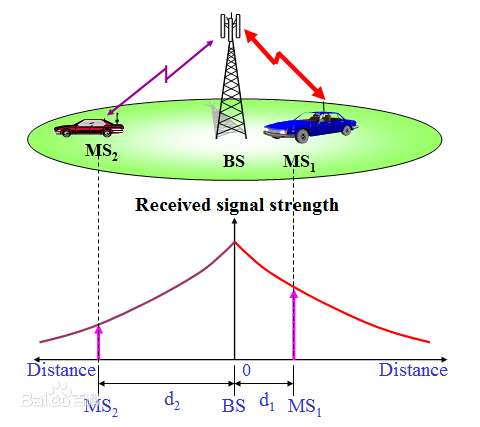
\includegraphics[width=0.50\textwidth]{img/yjxy.jpg}
  \caption{通信中的远-近效应示意图}
  \label{}
\end{figure}

也可以让伪卫星系统发射不同于卫星导航系统使用的测距码,这种新的测距码在旋转时应该考虑与原系统码族的互相关性,在此基础上改变一些参数,例如码率、顺序等。\upcite{04,001}

\subsubsection{多径效应}

多径效应由信号的反射引起。在伪卫星应用中,由于应用场景多在室内,所以能造成干扰的物体比较多(如墙壁、椅子、摆件等),而且伪卫星本身也是反射信号,多径效应就会造成一个信号偏移量,影响定位的精度。\upcite{002}在静态条件下,可以得到一个描述信号偏移的常向量,但在动态情况下,偏移量将是随机的。优化多径效应带来的影响将是伪卫星技术应用过程中的一个重点。现有的解决多径效应的主要途径是:对数据进行滤波和自适应处理;对天线进行改进;选择最优的星座布局和接收机的位置;改进硬件设计(由接收机,接收机天线和伪卫星信号发射器天线组成)。\upcite{001}

\subsubsection{大气层时延}

跟卫星导航系统相同的一点是:伪卫星信号在传输过程中也会受到大气层的影响,区别在于GNSS系统受到的大气延时影响包括电离层时延和对流层时延,而伪卫星系统由于布设高度较低,主要只受到对流层时延的影响。现在的做法是使用各种模型/函数来校准时延,例如GPS信号通常使用Saastamoinen、Black或者Hopfield模型来修正对流层时延的影响,但是这些模型的使用都非常依赖仰角。\upcite{001,05}现有解决模型包括:Hein所建立的一种函数模型,把大气折射率作为一个气象参数来刻画,这个模式要求对大气气压、温度、湿度精密测量,得出局地天气条件对于函数的作用;Barltrop等人提出了一种自适应对流层延迟估计算法。这种方法在定位解算时,以对流层延迟为额外未知参数,该方法可应用于卫星定位误差的补偿;RTCA提出的飞机精密进场和着陆的LASS的RTCA模型及Biberger等人对其的修改版;Bouska等人提出的Bouska模型。\upcite{002}

\subsection{结束语}

总的来说,伪卫星技术重在其灵活性、可移植性,使得我们有了与各种导航系统组合、集成、取长补短的可能性。尽管仍然存在一些局限性和疑难问题,但仍是应用前景广阔的一项技术。这一种互补的思想不仅在卫星导航领域,而且在各个学科都是十分常见的东西,例如计算机科学中的多级缓存,冲压、涡喷、涡扇、涡桨等多种飞机发动机。可以说,伪卫星技术的成功应用更启发我们在生活和以后的学习研究中将领域内的不同技术特点相互结合、改进,起到填补空白的目的。

最后请允许我赘言几句。这是作者本人进入大学的第一年,起初只是乘着对卫星、宇航的一些“不明觉厉”选修了杨宜康老师的“卫星导航技术漫谈”这门课,但是在课程开展之后,这门课程就深深吸引了我。杨老师在课堂上对于一些我们曾经只在《新闻联播》里听过的词汇侃侃而谈,也深入浅出、不失幽默地讲解了让非本专业和大一新生望而却步的技术原理,同时还能在需要严谨时将数学公式和物理方程信手拈来。我觉得这才应该是我心目中大学学习应有的样子。当然我也清楚,这只是一门“漫谈”的通识课,想要真正做到专业、渊博,少不了像杨老师一样长期的学习和研究,但这也确实吸引同为电信专业的我为之学习更多。

所以,最后还是感谢杨老师在短短半个学期的时间里给我们呈现的精彩课程!

%%%%%%%%%%%%%%%%%%%%%%%%%%%%%%%%%%%%%%%%%%%%%%%%%%%%%%%%%%%%%%%%%%%%%%%%%%%
%   使用BibTex管理参考文献

\bibliographystyle{IEEEtran}
\bibliography{thisbib}
%%%%%%%%%%%%%%%%%%%%%%%%%%%%%%%%%%%%%%%%%%%%%%%%%%%%%%%%%%%%%%%%%%%%%%%%%%%
%   创造附录
%\begin{appendices}
%    \renewcommand{\thesection}{\Alph{section}}
%    \section{附录标题}
%        这里是附录. 
%\end{appendices}

%%%%%%%%%%%%%%%%%%%%%%%%%%%%%%%%%%%%%%%%%%%%%%%%%%%%%%%%%%%%%%%%%%%%%%%%%%%
\end{document}
%%%%%%%%%%%%%%%%%%%%%%%%%%%%%%%%%%%%%%%%%%%%%%%%%%%%%%%%%%%%%%%%%%%%%%%%%%%